\section{Pistepilvet}\label{pistepilvet}

Pistepilville on useita käyttökohteita, joista arkkitehtuuri ja rakentaminen ovat tärkeimpiä. Pistepilvien hyödyntäminen voidaan aloittaa hyvin varhaisessa vaiheessa rakennusprojektia. Rakennettavan tontin ympäristöstä voidaan ottaa laserkeilauksia, jotta suunniteltavan rakennuksen sopimista tontille voidaan helposti arvioida. Rakennusprojektin aikana säännöllisesti tehdyillä laserkeilauksilla voidaan seurata tarkasti projektin etenemistä ja havaita mahdollisia ongelmia ajoissa. Pistepilvillä on myös tärkeä rooli rakennuksen valmistumisen jälkeen, sillä muutostöitä tehtäessä halutaan rakennuksesta saada ajantasalla oleva 3d-malli. Manuaalinen mallintaminen olisi hyvin työlästä verrattuna muutaman kymmenen pistepilven mittaamiseen laserkeilaimella, mikä voidaan tehdä päivässä. \cite{bim} 

Eräs mielenkiintoinen sovelluskohde laserkeilaukselle on siltojen rakentaminen. Sillanrakennuksessa haasteita tuottavat tien ja maaston geometrian yhteensovittamisen lisäksi projektin pitkä kesto. Silta on rakennettava osissa ja lopputulokseen kohdistuu tiukkoja turvallisuusvaatimuksia, minkä takia siltatyömaalla suoritetaan usein tarkistusmittauksia. Älykäs silta -projektissa tutkittiin tapoja hyödyntää tietotekniikkaa sillanrakentamisessa ja -korjaamisessa, ja havaittiin laserkeilauksen olevan hyvä tapa suorittaa tarkkuusmittauksia. Laserkeilauksella mitattiin pistepilviä sillan kannesta ja rakenteista, jonka jälkeen niistä muodostettiin pintoja 3d-suunnitteluohjelmaan. Pistepilvi ja siitä muodostettu geometria on esitetty kuvassa \ref{silt}. \cite{silta}   

\begin{figure}
    \centering
    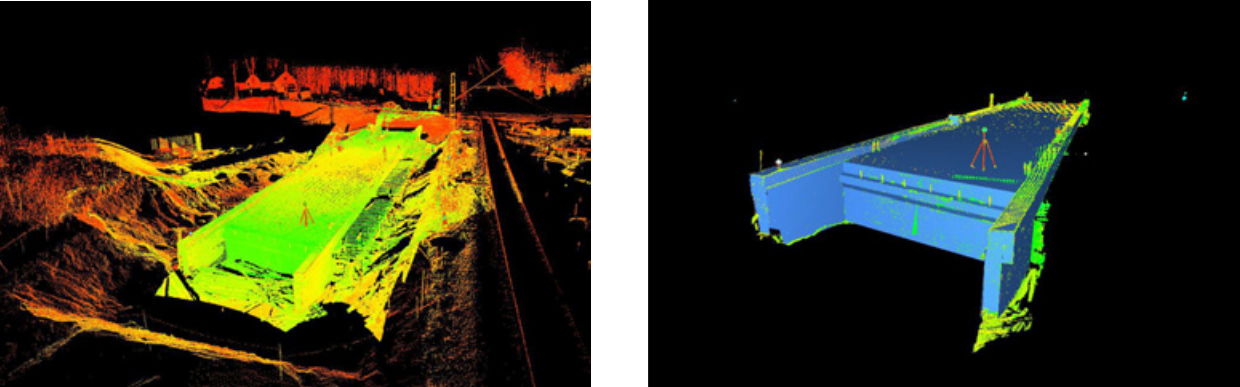
\includegraphics[width=\textwidth]{img/silta.png}
    \caption{Silta Joroisten ja Varkauden välissä Kuvasintiellä. Vasemmalla pistepilvi, oikealla pistepilvestä muodostetua geometriaa suunnitteluohjelmassa. \cite{silta}}
    \label{silt}
\end{figure}

Pistepilviä käytetään hyväksi myös arkeologiassa. Roomalaiset perustivat vuoden 40 tienoilla Tonavan varrelle nykyisen Itävallan alueelle
sotilasleirin, josta kasvoi myöhemmin Carnuntumin kaupunki. Kaupungin muurien ulkopuolelle rakennettiin amfiteatteri, johon mahtui 13 000 katsojaa.
Vuonna 2007 Ala-Itävallan osavaltion hallitus aloitti amfiteatterin alueella arkeologiset kaivaukset, joiden yhteydessä alueesta muodostettiin kattava pistepilvi noin kahdellasadalla laserkeilauksella. Ruudunkaappaus kyseisestä pistepilvestä on esitetty kuvassa \ref{amfi}. \cite{Carnuntum}

\begin{figure}
    \centering
    \includegraphics[width=0.7\paperwidth]{img/amphitheatre.png}
    \caption{Carnuntumin kaupungin amfiteatteri taltioituna laserkeilauksella. \cite{Amphitheatre}}
    \label{amfi}
\end{figure}

\begin{figure}
    \centering
    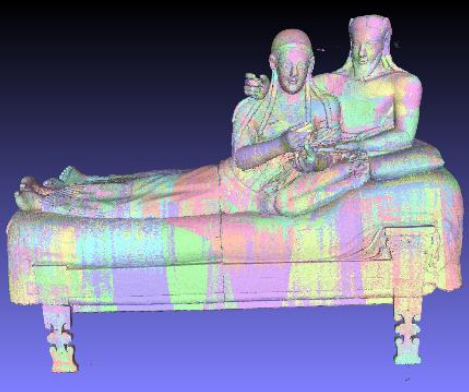
\includegraphics[width=0.4\paperwidth]{img/sarkofagi.png}
    \caption{Etruskilaisesta sarkofagista muodostettu pistepilvi. \cite{sarkofagi}}
    \label{sarko}
\end{figure}

Pistepilviä käytetään historiallisen kulttuuriperinnön säilyttämiseen myös pienemmässä mittakaavassa. 1800-luvulla tehdyissä Cerveterin arkeologisissa kaivauksissa Italiassa löydettiin 500-luvulla terrakottasavesta tehty etruskilainen sarkofagi, joka kuvasi avioparia rentoutumassa tuonpuoleisessa. Satoihin palasiin hajonnut sarkofagi restauroitiin vuonna 1893 ja se digitoitiin käyttämällä laserkeilausta ja fotogrammetriaa vuonna 2013 taidenäyttelyä varten. Sarkofagista keilattu pistepilvi on esitetty kuvassa \ref{sarko}. \cite{sarkofagi} 

Eräs vaativa pistepilvien sovelluskohde on itseohjautuvat kulkuneuvot. Voidakseen navigoida liikenteessä itseohjautuva auto tarvitsee kameroiden ja ultraäänisensoreiden lisäksi katolleen laserkeilaimen, jolla voidaan tarkkailla auton etäisyyttä muihin tienkäyttäjiin ja esteisiin. Itseohjautuvat autot ovat merkittävä tutkimuskohde myös pistepilvien käsittelyn kannalta. Auton katolle asennettavan laserkeilaimen tulisi olla tarkka, nopea ja edullinen, ja sen tuottamaa pistedataa täytyy voida käsitellä reaaliajassa. \cite{car} 

Pistepilviä voidaan käyttää myös huomattavasti suuremmassa mittakaavassa. Maanmittauslaitos on kerännyt ilmasta käsin pistepilvidataa lähes koko Suomen maaperästä. Lentokoneesta keilattu pistepilvi on melko harva — puoli pistettä neliömetriä kohden — mutta keilattavan kohteen laajuus tekee pilvistä valtavia. Pistepilviä on käytetty lähinnä metsävarojen kartoittamiseen, mutta Maanmittauslaitos aikoo ryhtyä keräämään pistedataa tarkemmilla laserkeilamilla myös rakennuksista. \cite{hs}

Laserkeilauksen kohteena ei ole aina maasto tai eloton rakennelma, vaan myös ihmisistä voidaan tehdä pistepilviä. Esimerkiksi moottoripyöräkypärien suunnittelija voi käyttää hyväkseen ihmisen päätä kuvaavia pistepilviä selvittääkseen sopivan muodon kypärän sisukselle. Kypärän ulkokuori voidaan sen jälkeen mallintaa suunnitteluohjelmistolla niin, että se täyttää tarvittavat turvallisuusvaatimukset. Pistepilvillä on paikkansa myös lääketieteessä. Proteesin valmistaja voi esimerkiksi käyttää potilaan terveestä jalasta mitattua pistepilveä suunnitellessaan proteesia, jotta se muistuttaisi mahdollisimman paljon amputoitua jalkaa. Myös kirurgit voivat käyttää leikkauksen suunnittelussa hyväkseen elimistä laserkeilauksella muodostettuja 3d-malleja. \cite{saxena}  



\subsection{Pistepilvien käsittely}\label{workflow}

Perinteinen pistepilvien mittaamiseen käytetty laserkeilain on jalustalla seisova laite, joka pyörii pystyakselinsa ympäri ampuen ympärilleen miljoonia laserpurskeita. Laserkeilain mittaa etäisyyksiä pisteisiin, joista laserpurske heijastuu takaisin keilaimeen ja muodostaa näistä pisteistä pistepilven. Heijastuksen voimakkuutta käytetään usein määräämään pisteelle väri. Yleensä tarkasteltavaa kohdetta täytyy keilata useista eri suunnista, jotta saataisiin tarpeeksi kattava joukko pistepilviä. Kohteesta riippuen voidaan tarvita jopa satoja keilauksia.

\begin{figure}
    \centering
    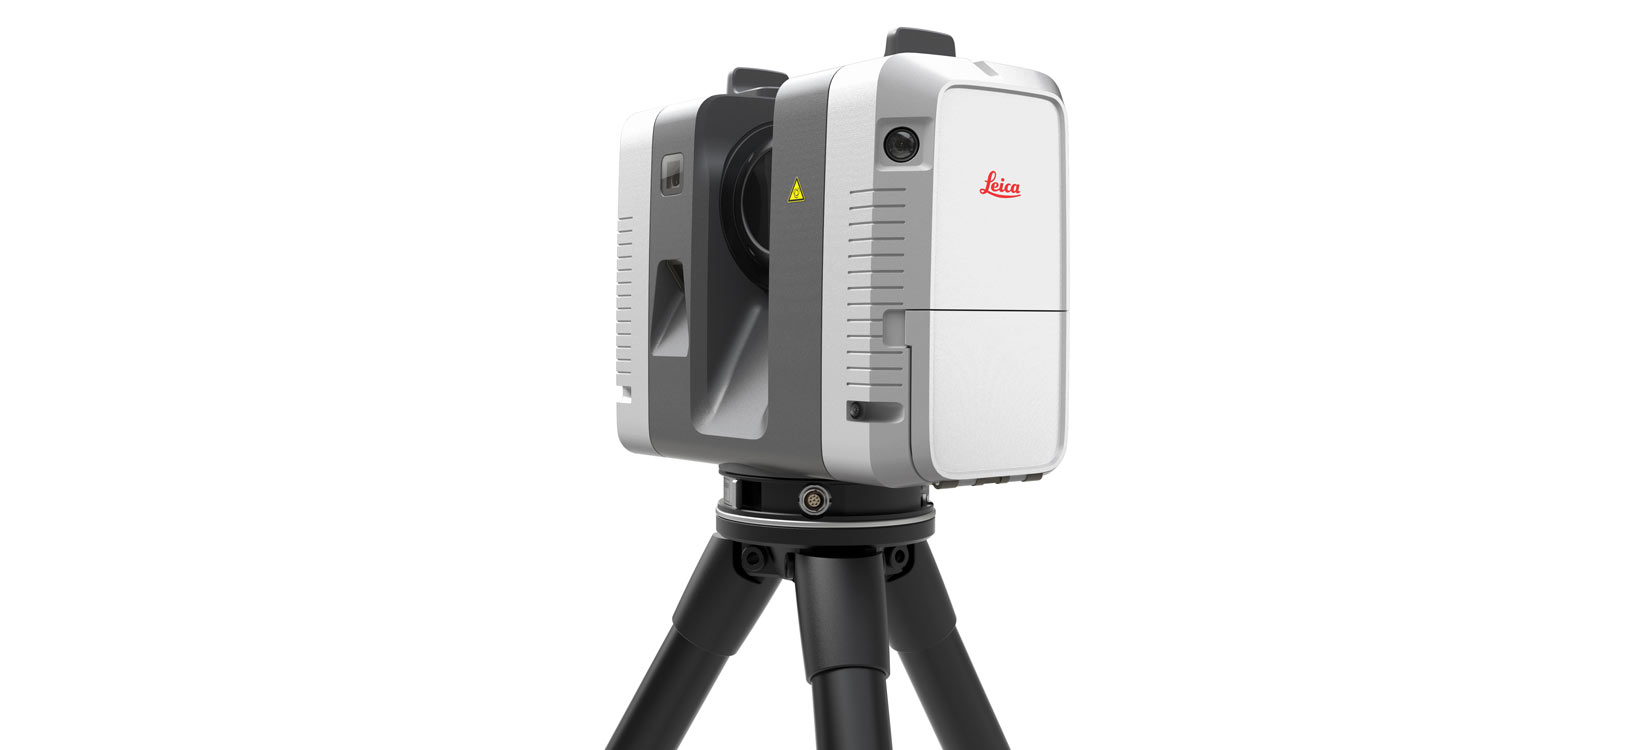
\includegraphics[width=0.7\paperwidth]{img/leica.jpg}
    \caption{Kulkuaikatekniikkaan perustuva Leica RTC360 -laserkeilain. \cite{skannerikuva}}
    \label{leica}
\end{figure}

Nykyaikaisella laserkeilaimella saadaan muodostettua hyvin tarkka ja tiheä pistepilvi nopeasti. Esimerkiksi kuvassa \ref{leica} näkyvän Leica Geosystemsin RTC360 -keilaimen luvataan mittaavan jopa kaksi miljoonaa pistettä sekunnissa ja kiertävän täyden ympyrän alle kahdessa minuutissa. Keilaimen lisäksi laitteessa on digitaalinen kamera, jolla saadaan määritettyä pisteille oikeat värit. \cite{leica} 

Laserkeilaimien toimintaperiaatteissa on eroja. Kaksi yleisintä toimintaperiaatetta ovat kulkuaikatekniikka \engl{time-of-flight} ja vaihesiirtotekniikka \engl{phase shift}. Kulkuaikatekniikkassa pisteen etäisyys keilaimesta selviää ajasta, joka kuluu laserpurskeen lähetettämisestä sen heijastuksen vastaanottamiseen. Pisteen etäisyys keilaimesta lasketaan yksinkertaisesti kaavalla 
\begin{equation}
    d=\frac{c\cdot t}{2},    
\end{equation}
missä $c$ on valonnopeus ja $t$ on mitattu aika. 
Vaihesiirtotekniikka perustuu keilaimesta lähtevän signaalin vaiheen vertaamista palaavan signaalin vaiheeseen. Pisteen etäisyys keilaimesta saadaan laskemalla 
\begin{equation}
    d=n\cdot \lambda + \frac{\Phi \cdot \lambda}{2 \cdot \pi},
\end{equation}
missä $n$ on havainnon täysien aaltojen määrä, $\lambda$ on signaalin aallonpituus ja $\Phi$ on lähtevän ja palaavan signaalin vaihe-ero. \cite{fabritius}

\begin{figure}
    \centering
    \subfile{fig/pallo.tex}
    \caption{Pallokoordinaatisto. Pisteen sijainti avaruudessa ilmaistaan korotuskulmalla $\theta$, atsimuuttikulmalla $\phi$ ja säteellä $r$.}
    \label{pallo}
\end{figure}{}

Laserkeilain tallentaa mittaamansa pisteen pallokoordinaateissa. Pisteen siirtäminen pallokoordinaateista karteesiseen koordinaatistoon onnistuu laskemalla koordinaatit 
\begin{equation}
    \begin{split}
        x&=r \cdot \sin \theta \cdot \cos \phi,\\ 
        y&=r \cdot \sin \theta \cdot \cos \phi,\\
        z&=r \cdot \cos \theta,    
    \end{split}
\end{equation}
missä r on pallon säde, $\theta$ on korotuskulma ja $\phi$ atsimuuttikulma. Pallokoordinaatistoa on havainnollistettu kuvassa \ref{pallo}.

Laserkeilauksella tuotettuja pistepilviä ei usein käytetä sellaisenaan, vaan niitä täytyy ensin esikäsitellä. Yleisiä esikäsittelyvaiheita ovat panoramakuvien luominen, usean pistepilven rekisteröinti yhteen koordinaatistoon, muukalaispisteiden poistaminen ja pintojen rekonstruointi.

Yksinkertaisin tapa visualisoida pistepilvi on muodostaa siitä kaksiulotteinen kuva. Pilvestä voidaan luoda panoramakuva projisoimalla laserkeilaimen ympäröimät pisteet kaksiulotteiselle kuvatasolle.\footnote{Projektio vaikuttaa suuresti panoramakuvan laatuun. Hyvän yleiskatsauksen erilaisiin projektiohin antaa \cite{proj}. Kuvassa \ref{img:pano} on käytetty tasavälistä lieriöprojektiota \engl{equirectangular projection}.} Kuvakoosta riippuen voidaan pistepilvestä karsia huomattava määrä pisteitä, joiden koko olisi liian pieni kuvatasolle projisoituna. Panoramakuvat toimivat siis myös pistedatan pakkausalgoritmina. Panoramakuvan pikseleille voidaan määrittää värit joko sen perusteella, kuinka paljon valoa heijastuu takaisin niitä vastaavista pilven pisteistä, kuinka kaukana pisteet ovat keilaimesta tai kuinka korkealla pisteet ovat maanpinnasta. Panoramakuvaan on helppo soveltaa erilaisia kuvankäsittelyalgoritmeja, kuten piirteentunnistusta \engl{feature detection}. Kuvassa \ref{img:pano} on esimerkki panoramakuvasta, joka on väritetty laserpurskeiden heijastuksien intensiteetin perusteella.

\begin{figure}
    \centering
    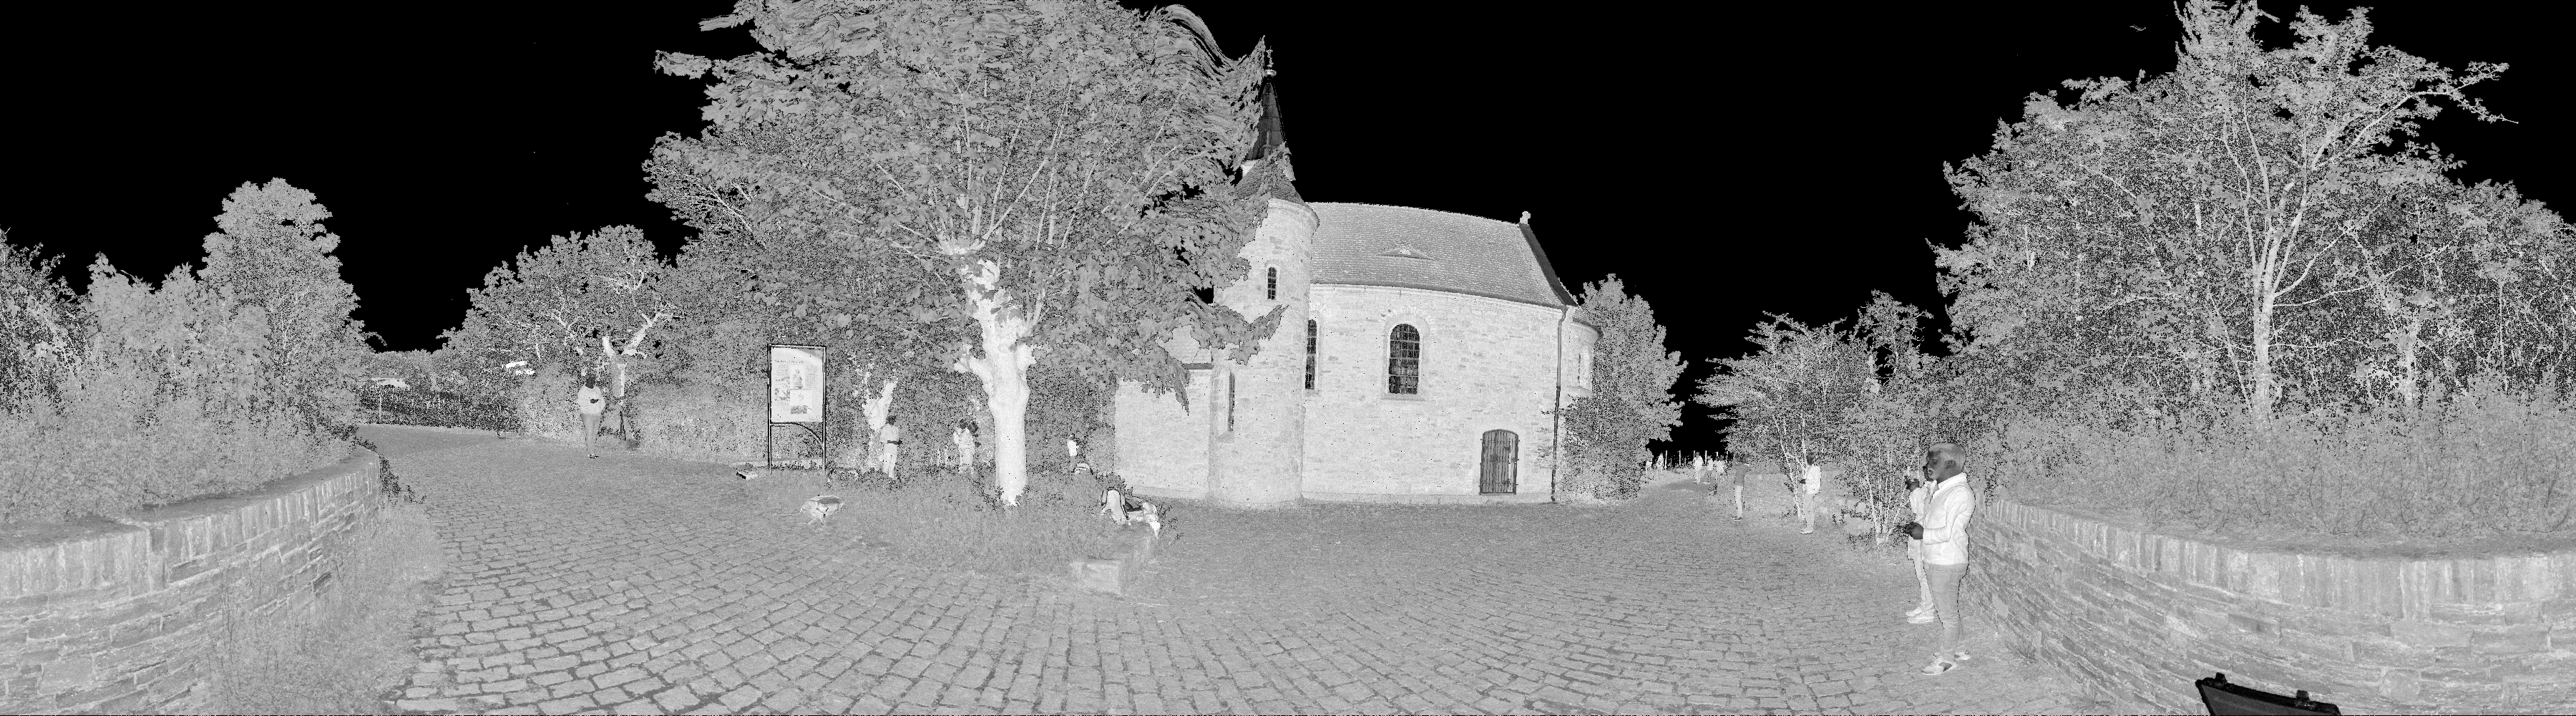
\includegraphics[width=\textwidth]{img/pano.png}
    \caption{Saksan Würzburgissa sijaitsevasta Randersackerin Neitsyt Marian kärsimysten kappelista keilatusta pistepilvestä muodostettu panoramakuva.}
    \label{img:pano}
\end{figure}

Laserkeilauksen tuottama pistepilvi sisältää joukon pisteitä pallokoordinaatistossa, jonka origona on keilaimen sijainti. Usein keilauksen kohteesta otetaan kymmeniä tai jopa satoja keilauksia, jotka täytyy saada samaan koordinaatistoon. Tätä sovittamista kutsutaan pistepilvien rekisteröinniksi. 

Pistepilviä voidaan rekisteröidä usealla eri tavalla. Joskus keilattavaan kohteeseen asetetaan erityisiä merkkikuvioita, jotka näkyvät useasta keilaimesta. Kun tiedetään merkkien etäisyys ja suunta kustakin keilaimesta, voidaan pistepilvet sovittaa helposti yhteen koordinaatistoon trigonometrian avulla. Joissakin sovelluksissa käyttäjä merkitsee kahdesta pilvestä joukon pisteitä, joiden avulla pilvet saadaan rekisteröityä. Esimerkiksi 3DTK-kirjastolla käyttäjä voi valita kahdesta pilvestä samaa aluetta kuvaavia pisteitä, joiden avulla pilvien yhteensovitus onnistuu automaattisesti \cite{3dtk}.  

\begin{figure}
    \centering
    \subfloat[]{
        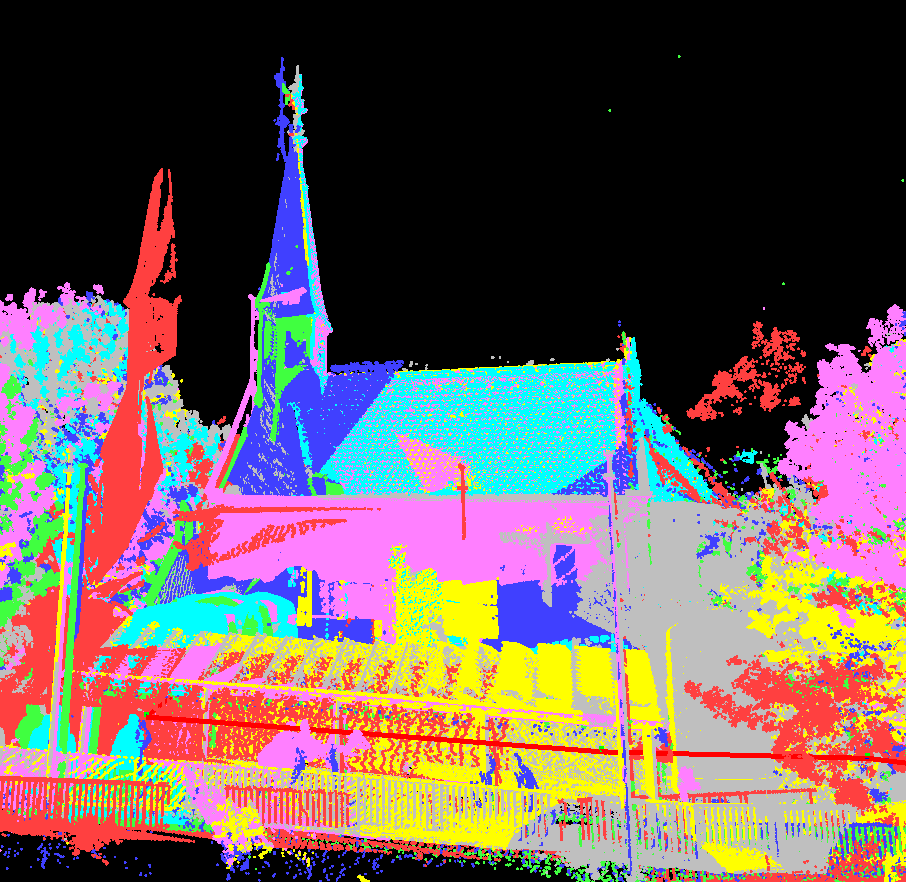
\includegraphics[width=.498\textwidth]{img/reg1.png}
    }
    \subfloat[]{
        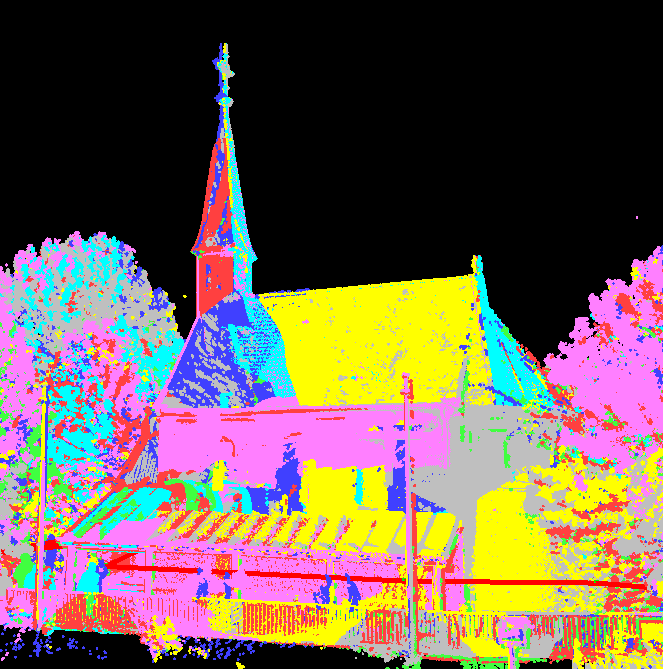
\includegraphics[width=.48\textwidth]{img/reg2.png}
    }%
    
    \caption{Kuvan \ref{img:pano} kappelista keilaittuja pistepilviä (a) ennen rekisteröintiä ja (b) rekisteröinnin jälkeen. Kunkin keilauksen pisteet on piirretty eri väreillä.}
    \label{img:reg}
\end{figure}

Pistepilviä voidaan rekisteröidä myös ilman merkkikuvioita tai käyttäjän apua. Iteratiivinen lähimmän pisteen algoritmi \engl{iterative closest point, ICP} sovittaa pistepilven toiseen etsimällä rotaation ja translaation, jolla pilvien välinen virhe saadaan minimoitua. Virheen laskemista varten täytyy määrittää pilvistä toisiaan vastaavat pisteet. Yksinkertaisimmillaan pistettä vastaavaksi pisteeksi valitaan toisesta pilvestä se, jonka euklidinen etäisyys edellä mainittuun on pienin. Iteratiivisen algoritmin kunkin transformaation sopivuus lasketaan kaikkien vastaavien pisteiden välisten etäisyyksien muodostamasta virheestä. Algoritmin iteroiminen voidaan lopettaa, kun jokin ennaltamäärätty raja virheelle on alitettu. Kuvassa \ref{img:reg} on ICP-algoritmilla sovitettu yhteen kuusi pistepilveä. \cite{icp}

%\footnote{Täysin automaattista pistepilvien rekisteröintiä on tutkittu paljon, ks. esim. \cite{Pascal}.} 

ICP-algoritmi tarvitsee kuitenkin käyttäjältä hyvän alkuarvauksen keilausten sijainneista yhteisessä koordinaatistossa, jotta virhe suppenisi ja pilvien sovittaminen onnistuisi. Se on myös erittäin raskas suorittaa isoille pistepilville. Yleensä ICP-algoritmia käytetäänkin karkeamman rekisteröintialgoritmin suorittamisen jälkeiseen hienosäätämiseen. Karkeampi pilvien yhteensovittaminen tehdään yleensä etsimällä kahdesta pistepilvestä muodostetuista panoramakuvista toisiaan vastaavia avainpisteitä \engl{keypoints}. Näiden avainpisteiden sijainneista saadaan harva joukko pisteitä, joiden yhteensovittaminen on paljon helpompaa kuin kokonaisten pistepilvien. Suosittuja tekniikoita avainpisteiden löytämiseen ovat esimerkiksi Harrisin nurkat \cite{harris} sekä FAST ja SIFT -piirteet \cite{fast}\cite{sift}. \cite{weinmann}

Joissakin sovelluksissa halutaan luoda pistedatasta kohteen pintoja kuvaava polygoniverkko, jotta visualisointi olisi nopeampaa nykyaikaisilla grafiikkakirjastoilla ja visuaalinen lopputulos parempi. Yksinkertainen tekniikka luoda tiivis kolmiointi pistepilvestä on Delaunayn kolmiointi. Delaunayn kolmiointi perustuu Voronoin diagrammiin \engl{Voronoi diagram}, joka jakaa pisteitä sisältävän tason tai avaruuden konvekseihin Voronoin soluihin. Voronoin solu kattaa sen alueen, jossa etäisyys solua vastaavaan pisteeseen on pienempi kuin muihin pisteisiin. Kahden solun välillä on Voronoin jana, josta etäisyys kahteen pisteeseen on sama, ja kolmen janan leikkauspisteessä on Voronoin kärki, josta etäisyys kolmeen pisteeseen on yhtä suuri. Delaunayn kolmiointi on Voronoin diagrammin duaaligraafi. Kolmiointi luodaan Voronoin diagrammista siten, että pisteiden välillä on kaari, mikäli niitä vastaavat Voronoin solut jakavat Voronoin janan. \cite{delaunay}

\begin{figure}
    \centering
    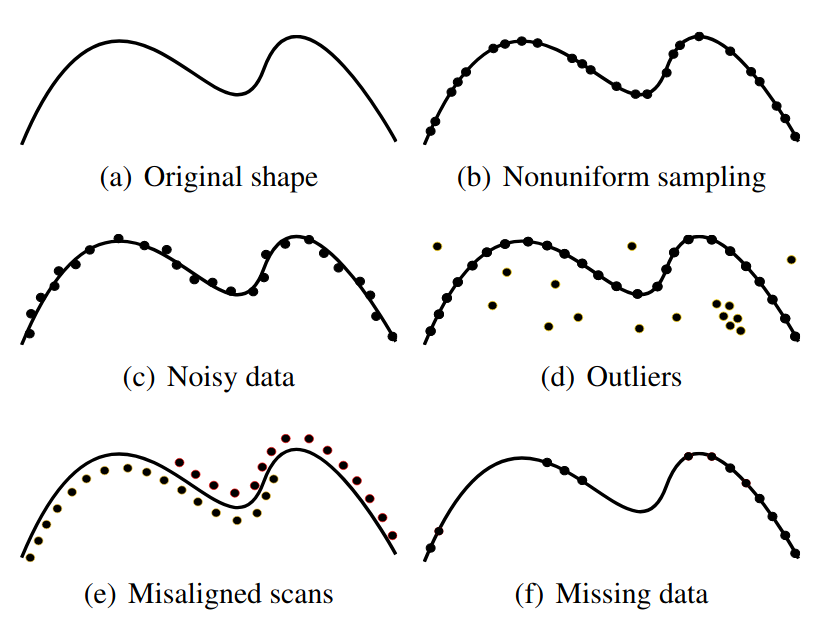
\includegraphics[width=0.7\textwidth]{img/artifacts.png}
    \caption{Kaarevasta pinnnasta (a) keilatussa pistepilvissä esiintyviä mahdollisia virheitä: (b) epätasainen pistetiheys, (c) häiriötä pisteiden sijainneissa, (d) muukalaispisteitä, (e) epätarkka rekisteröinti ja (f) puuttuvaa dataa. \cite{berger}}
    \label{img:artifacts}
\end{figure}

Oikeat, laserkeilaimella taltioidut pistepilvet sisältävät kuitenkin usein erilaisia virheitä, kuten kuvassa \ref{img:artifacts} esitellyt epätasainen keilaus, keilaimen häiriö, muukalaispisteet \engl{outlier}, ongelmat rekisteröinnissä ja puuttuva data. Virheiden johdosta Delaunayn kolmiointi ei ole kovin tehokas algoritmi kolmioverkon muodostamiseen pistepilvestä. Useissa pintojen rekonstruointialgoritmeissa tehdään joitakin oletuksia pistepilven ominaisuuksista. Etenkin tietokoneavusteisessa suunnittelussa keilauksen kohteet muodostuvat yksinkertaisista geometrisista primitiiveistä, kuten tasoista ja sylintereistä. Esimerkiksi RANSAC-algoritmi \cite{ransac} sovittelee primitiivejä satunnaistetusti pistepilveen ja arvioi niiden sopivuutta. \cite{berger} 

Joskus on hyödyllistä tietää pistepilven esittämien pintojen normaalivektorit. Tasainen pinta on helppo sijoittaa pistepilven päälle, jos jollakin alueella on tiheästi pisteitä, joiden normaalivektorit osoittavat samaan suuntaan. Laserkeilaimen epätarkkuudesta tai vaikkapa tuulen heiluttamista puiden lehdistä johtuen on pistepilvissä usein muukalaispisteitä. Yksinkertainen tapa havaita ja poistaa muukalaispisteitä on vertailla pisteiden normaalivektoreita niiden naapuruston normaaleihin ja etsiä poikkeavuuksia. 

Pisteen $p$ normaalivektori voidaan selvittää pääkomponenttianalyysillä \engl{principal component analysis, PCA}. Ensin on etsittävä pilvestä pisteen $p$ $k$ lähintä naapuria, jonka jälkeen naapuruston pisteistä lasketaan ominaisarvot. Kahta suurinta ominaisarvoa vastaavaa ominaisvektoria voidaan käyttää kuvaamaan tasoa, joka sovitetaan naapuruston päälle. Jäljelle jäävä ominaisvektori kuvaa pisteen $p$ normaalia. \cite{huang}

\subsection{Pistepilvien hyödyntäminen suunnitteluohjelmistoissa}\label{laitossuunnittelu}

Edellä mainittiin erilaisia sovelluksia laserkeilainten tuottamille pistepilville. Tässä tutkielmassa keskitytään pistepilvien hyödyntämiseen tietokoneavusteisessa suunnittelussa \engl{computer aided design, CAD} ja erityisesti laitossuunnitteluohjelmistoissa \engl{plant design software}.

Tietokoneavusteisessa suunnittelussa pistepilviä käytetään olemassaolevien rakenteiden taltiointiin. Usein käytetty esimerkki on autoteollisuuden alalta: ryhmä suunnittelijoita kokeilee uutta korimallia rakentamalla prototyyppiauton helposti muovattavasta materiaalista. Kun prototyyppi on todettu aerodynaamiseksi ja miellyttävän näköiseksi, täytyy se saada digitoitua, jotta se voidaan siirtää massatuotantoon. Usein yksinkertaisin ja kustannustehokkain tapa on laserkeilata prototyyppi ja jatkokäsitellä pistepilveä niin, että saadaan luotua haluttu 3d-malli.

Laitossuunnittelussa yleisempi ongelma on 3d-mallin vanhentuminen tai sen puuttuminen kokonaan. Vanhempien laitosten suunnitteluun on usein käytetty vain 2d-piirroksia tai pienoismalleja. Vaikka laitosta alunperin suunniteltaessa siitä olisi tehty 3d-malli, laitteistojen sommittelua saatetaan muuttaa ilman, että samoja muutoksia tehdään 3d-malliin. Kun 3d-mallia halutaan taas hyödyntää, voi olla kustannustehokkaampaa luoda laitoksesta laserkeilaimella pistepilvi kuin mallintaa tehdyt muutokset suunnitteluohjelmalla. \cite{Piipponen}

Kuten sillanrakennuksessa, myös laitoksia rakentaessa on joskus syytä suorittaa tarkastusmittauksia ja verrata niitä alkuperäiseen 3d-malliin. Laserkeilaus on tähänkin tarkoitukseen sopivia tekniikka, sillä pistepilvien tuottaminen on helppoa ja niitä pääsee tarkastelemaan nopeasti keilauksen jälkeen. Tarkkuudessakaan pistepilvet eivät häviä perinteisemmille mittaustavoille. Nykyaikaisten laserkeilainten tuottamat pistepilvet ovat niin tarkkoja, että niistä voi havaita esimerkiksi putkien roikkumisen ja lämpölaajenemisen \cite{Piipponen}. 

Pistepilvien pääasiallinen käyttötarkoitus laitossuunnittelussa on uudistustöiden suunnittelu. Muuttuneet tuotantotarpeet tai lainsäädäntö saattavat aiheuttaa tarpeen suurillekin muutostöille. Jos laitokseen täytyy esimerkiksi asentaa savukaasupesuri, voidaan laitoksen sisätiloista luoda pistepilvi, asettaa pesurin 3d-malliobjekti suunnitellulle paikalle ja reitittää tarvittavat hormit paikalleen. Tämän jälkeen voidaan tarkastaa, osuvatko malliobjektit pistepilven pisteisiin.  

%halutaan vaikkapa uusi vesiputki, voidaan sen mahtuminen varmistaa reitittämällä putki suunnitteluohjelmistolla ja tarkastamalla, osuuko se pistepilveen. Jos taas vanhasta laitoksesta halutaan luoda ajantasalla oleva, solidigeometriaa sisältävä 3d-malli, voi suunnittelija mallintaa laitosta pistepilvien avulla. Pistepilven päälle on helppo sijoittaa suunnitteluohjelman putkistoja ja laitteita oikeille paikoilleen. 

%Markkinoilla on myös ohjelmistoja, joiden luvataan tuottavan pistepilvestä automaattisesti älykäs 3d-malli komponenttitietoineen ilman aikaavievää päällemallinnusta \cite{aveva}. 

Usein pistepilvellä kuvattu laitos halutaan muuntaa suunnitteluohjelmiston käyttämäksi solidigeometriaksi. Lattiat ja seinät on tasoina helppo asettaa paikalleen, kuten myös suunnitteluohjelmiston komponenttikirjastosta löytyvät laitteet. Suurin työ on yleensä putkistoissa, ilmakanavissa ja kaapeliradoissa. Useat suunnitteluohjelmistot tarjoavat jonkinasteista automatisointia etenkin putkien reititykseen pistepilven päälle. Ohjelmisto voi automaattisesti tunnistaa pilvestä sylintereitä ja asettaa niiden päälle sopivia putkisto-osia. Vaihtoehtoisesti käyttäjä voi valita pilvestä muutamia pisteitä ja ohjelmisto laskee niiden perusteella putken pituuden ja halkaisijan ja asettaa oikean osan paikalleen. Markkinoilla on myös ohjelmistoja, joiden luvataan tuottavan pistepilvestä automaattisesti älykäs 3d-malli komponenttitietoineen \cite{aveva}. 

Huomattava osa suunnittelutyöstä koostuu putkistojen reitityksestä ja putkien tunnistamista pistepilvistä onkin tutkittu paljon. Ahmed, Haas ja Haas (2013) ehdottavat Hough-muunnokseen \engl{Hough-transform} perustuvaa tekniikkaa putkistojen automaattiseen tunnistukseen pistepilvestä. Tekniikka vaatii toimiakseen käyttäjältä syötteenä laserkeilattujen putkien ominaisuuksia, kuten putkien suunnan pistepilven koordinaatistossa, putkien säteet ja niiden määrän. Pistepilvi jaetaan ensin ohuihin siivuihin, jotka jakavat syötteenä annettuun suuntaan kulkevat putket lyhyihin pätkiin. Pisteet projisoidaan kaksiulotteiselle kuvatasolle jossa ne kuvataan ympyröinä, joiden halkaisija on sama kuin potentiaalisten putkien poikkileikkaus. Näiden ympyröiden leikkauspisteet selvitetään ja putken keskilinjoiksi tulkitaan ne kohdat, joissa on eniten ympyröiden leikkauspisteitä. \cite{ahmed}

Liu et al. (2013) esittelivät samankaltaisen lähestymistavan, jossa ongelma redusoitiin ympyröiden sovittamiseksi pisteisiin. \cite{liu} Toteutus pystyi kuitenkin havaitsemaan vain vaakatasossa ja pystysuorassa kulkevat putket. Qiu, Zhou, ja Neumann (2014) esittelivät tekniikan, joka löytää myös viistossa kulkevat putket ja pystyy yhdistämään putkia linjastoiksi asettamalla niiden väliin mutka- ja haaraosia. Algoritmi ei vaadi lähtöoletuksia pistepilvestä mutta pisteiden normaalivektorit täytyy olla selvillä. Pistepilvi jaetaan ensin piempiin kuutioihin joista etsitään putkien mahdollisia kulkusuuntia valitsemalla satunnaisten pisteiden normaalivektorien kanssa kohtisuora vektori ja laskemalla kuinka monen muun pisteen normaalivektorit ovat sen kanssa kohtisuoria. Vektori tulkitaan putken keskilinjaksi kun tarpeeksi monen pisteen normaalivektorit ovat sen kanssa kohtisuorassa. Seuraavaksi putkien paksuudet selvitetään litistämällä pisteet keskilinjojen suuntaisesti tasoon, minkä jälkeen pistepilven päälle voidaan sovittaa putkia kuvaavia sylintereitä. Lopuksi sylinterien päihin sovitetaan sopivia liitososia. \cite{qiu}

%Tietokoneavusteisen suunnittelun ohjelmisto käsittelee pistepilviä eri tavoin riippuen suunnittelutyön luonteesta. Kappalemallinnuksessa visualisoidaan usein yksittäisiä osia, joita kuvaavat pistepilvet ovat hyvin tiiviitä ja usein kaikki pisteet ovat kerralla näkyvissä. Laitossuunnittelussa pistepilvet ovat taas hyvin laajoja ja voivat kuvata esimerkiksi kokonaista tehdasaluetta. Näissä sovelluksissa on tärkeää pistepilven nopea rajaaminen niin, että vain näkymän sisältävät pisteet visualisoidaan. Usein on tarpeen myös käyttää eri tarkkuuksia pistepilven eri osille; kaukana katsojasta sijaitsevista pisteistä piirretään vain osa \cite{mikko}. 

\subsection{Pistepilvien visualisoinnin haasteet}

Suurin haaste pistepilvien käsittelyssä ja visualisoinnissa on niiden koko. Nykyaikainen laserkeilain, kuten aiemmin esitetty Leica Geosystemsin RTC360, tuottaa satoja miljoonia pisteitä sisältävän pistepilven. Kun tällaisella keilaimella tehdään useita keilauksia, on pisteiden määrä valtava. Oletetaan esimerkiksi, että suuressa projektissa käytetään pistepilviä, joissa on yhteensä miljardi pistettä. Kun koordinaatit tallennetaan kolmella nelitavuisella liukuluvulla ja värit RGB-muodossa kolmella tavulla ja lisätään perään vielä yksi täytetavu, voidaan yksi pilven piste esittää 16:lla tavulla. Miljardin pisteen pilvi olisi siis kooltaan 16 gigatavua mahdollisen metadatan lisäksi. Tämän kokoista pilveä ei haluta pitää kerralla keskusmuistissa, vaan pisteitä tulisi hakea levyltä muistiin vain tarvittaessa. 

Pisteiden tallentaminen levylle aiheuttaa kuitenkin ongelmia tiedonsiirron hitauden takia, sillä tiedonsiirtonopeus kiintolevyltä on jopa kaksi kertaluokkaa hitaampi kuin keskusmuistista. Ongelman ratkaisemiseksi käytetään usein ulkoisen muistin algoritmeja \engl{out-of-core algorithm}, jotka lataavat pisteitä levyltä muistiin isoissa palasissa, mikä on huomattavasti nopeampaa kuin yksittäisten pisteiden lataaminen. \cite{scheiblauer} 

Pistepilvien koon vuoksi ei ole realistista olettaa, että kaikki pisteet voitaisiin visualisoida reaaliajassa.\footnote{Miellyttävän käyttökokemuksen takaamiseksi pitäisi ruutu päivittää vähintään kymmenen kertaa sekunnissa.} Tästä syystä on kehitetty erilaisia tekniikoita pistepilven harventamiseen ja osittaiseen piirtämiseen. Yksinkertainen tapa harventaa pistepilveä on jakaa sen peittämä alue niin kutsuttuihin vokseleihin \engl{volume element, voxel}, eli säännöllisiin kuutioihin, ja visualisoimalla vain yksi piste kustakin vokselista. Pilven harventaminen kuitenkin aiheuttaa yksityiskohtien katoamista pilvestä, joten sitä täytyy käyttää sovelluskohteesta riippuen maltillisesti. 

Toinen keino vähentää visualisoitavien pisteiden määrää on määrittää pistepilvelle tarkkuustasot \engl{level-of-detail, LOD}. Tarkkuustasot mahdollistavat pistepilven astettaisen tarkentamisen karkeasta yleiskuvasta yksityiskohtiin. Usein interaktiivisissa ohjelmistoissa korkean ruudunpäivitystaajuuden ylläpitäminen vaatii sitä, että pistepilvi piirretään matalimmalla tarkkuudella esimerkiksi käyttäjän pyörittäessä näkymää. Toisaalta kun kamera pysähtyy paikalleen, voidaan visualisointiin käyttää enemmän aikaa ja pistepilveä tarkentaa.